\documentclass[a4paper, 12pt]{article}

\usepackage{hyperref}
\usepackage{fullpage}
\usepackage[top=0.5in, bottom=1.5in, left=0.5in, right=0.5in, footskip=4em]{geometry}
\usepackage{amsmath}
\usepackage{fancyhdr}
\usepackage[usenames,dvipsnames]{xcolor}
\usepackage{pgfornament}

\usepackage[shortlabels]{enumitem}
\usepackage{xspace}
\usepackage{lastpage}
\usepackage{multicol}
\usepackage{blindtext}
\usepackage{titling}
\usepackage{standalone}
\usepackage{amsfonts}
\usepackage[framemethod=TikZ]{mdframed}
\usetikzlibrary{calc}
\usepackage{lineno}
\usepackage{amsthm}
\usepackage{amssymb}
\usepackage{mathtools}
\usepackage{datetime}
\usepackage[most]{tcolorbox}
\usepackage{cancel}
\usetikzlibrary{tikzmark}
\usepackage{pgfplots}
\linenumbers


%BEGIN_FOLD Commands
\newcommand{\half}{\frac{1}{2}}
\newcommand{\epv}[1]{\ensuremath{\left< #1 \right>}\xspace}
\newcommand{\variance}{\ensuremath{\text{Var}}}
\newcommand{\eout}{\ensuremath{E_\text{out}}\xspace}
\newcommand{\ein}{\ensuremath{E_\text{in}}\xspace}
\newcommand{\cx}{\ensuremath{\mathcal{X}}\xspace}
\newcommand{\cz}{\ensuremath{\mathcal{Z}}\xspace}
\newcommand{\real}{\mathbb{R}}
\DeclareSymbolFont{extraup}{U}{zavm}{m}{n}
\DeclareMathSymbol{\varheart}{\mathalpha}{extraup}{86}
\DeclareMathSymbol{\vardiamond}{\mathalpha}{extraup}{87}
\renewcommand{\heartsuit}{\textcolor{red}{\varheart}}
\renewcommand{\diamondsuit}{\textcolor{red}{\vardiamond}}
\newcommand{\definition}{\vspace{1em}\noindent\textbf{Def:} }
\newcommand{\theorem}{\vspace{1em}\noindent\textbf{Theorem:} }
\newcommand{\example}{\vspace{1em}\noindent\textbf{Example:} }
\newcommand{\predicate}{\vspace{0.25em}\noindent\textbf{Inductive Predicate:} }
\newcommand{\inductivestep}{\vspace{0.25em}\noindent\textbf{Inductive Step:} }
\renewcommand{\proof}{\vspace{0.5em}\noindent\textbf{Proof:} }
\newcommand{\lemma}{\vspace{1em}\noindent\textbf{Lemma:} }
\newcommand{\hint}{\textbf{Hint:} }
\newcommand{\basecase}{\vspace{0.25em}\noindent\textbf{Base Case:} }
\newcommand{\inductivehypothesis}{\vspace{0.25em}\noindent\textbf{Inductive Hypothesis:} }
\newcommand{\collorary}{\vspace{1em}\noindent\textbf{Collorary:} }
\newcommand{\qedd}{\qed\newline}
\newcommand{\kwd}[1]{\textcolor{blue}{\textbf{\underline{#1}}}}
\newcommand\ColorBox[2][]{%
	\stepcounter{mybox}%
	\node[draw=red!70!black,fill=red!20,align=left,#1] (box\themybox) {#2};
}
\newcommand{\expl}[2]{%
	\underset{\substack{\uparrow\\\mathrlap{\text{\hspace{-1em}#2}}}}{#1}}
\newcommand{\uexpl}[2]{%
	\overset{\substack{\mathrlap{\text{\hspace{-1em}#2}}\\\downarrow}}{#1}}
\newcommand{\st}{\text{ such that }}
\newcommand{\R}{\textcolor{red}{R}}
\newcommand{\sumn}{\sum^n_{i=0}}
\newcommand{\sumxn}{\sum^n_{x=0}}
\newcommand{\red}[1]{\textcolor{red}{#1}}
\newcommand{\blue}[1]{\textcolor{blue}{#1}}
%\newcommand{\qed}{\ensuremath{\blacksquare}}
%END_FOLD
\newcommand{\sidenote}[1]{\textcolor{gray}{#1}}

%BEGIN_FOLD miscellaneious default
\makeatletter
% Make a copy of macros responsible for entering display math mode
\let\start@align@nopar\start@align
\let\start@gather@nopar\start@gather
\let\start@multline@nopar\start@multline
% Add the "empty line" command to the macros
\long\def\start@align{\par\start@align@nopar}
\long\def\start@gather{\par\start@gather@nopar}
\long\def\start@multline{\par\start@multline@nopar}
\makeatother
\setlength{\columnsep}{1cm}
%opening
\setlength{\abovedisplayskip}{-\baselineskip}%
\setlength{\abovedisplayshortskip}{\abovedisplayskip}%

\pagestyle{fancy}
\renewcommand{\headrulewidth}{0pt}
\lfoot{\small{\course}: Week \weekno}
\rfoot{\small{\thetitle}}
\rhead{}
\cfoot{\pgfornament[height=1em, ydelta=-0.4em]{17} \thepage of \pageref{LastPage}  \pgfornament[height=1em, ydelta=-0.4em]{18}}

\DeclareMathOperator{\sign}{sign}
\newcommand{\vect}[1]{\ensuremath{\mathbf{#1}}\xspace}

\tikzstyle{every picture}+=[remember picture]
\newcommand{\bwgrid}[1]{
	\def \aaa #1
	
	\foreach \y in {0,1,2} {
		\foreach \x in {0,1,2} {
			\pgfmathsetmacro{\clr}{\aaa[\x][\y]}
			%\message{aaa \clr}
			\definecolor{MyColor}{rgb}{\clr,\clr,\clr}
			\path[fill=MyColor] (\x,\y) rectangle ++(1,1); 
		}
	}
	\draw[step=1cm,very thin] (0,0) grid (3,3);	
}

\setenumerate{label=\alph*.)}
\definecolor{db}{RGB}{100,65,23}

%END_FOLD

\newcommand{\course}{Discrete Math}
\title{Recurrence}
\newcommand{\weekno}{5}

\begin{document}
\begin{center}
	\textcolor{orange}{\textsc{\course}}\\
	\huge\textbf{\textsc{\thetitle}}\\
	\small\textcolor{gray}{Last updated:\, \today \, \currenttime}\\
	\pgfornament[width=0.7\textwidth, color=white!30!black]{88}
\end{center}

\begin{multicols}{2}
\section*{Tower of Hanoi}
Consider the following game of $n$ circular disks of different size and three poles. At the start of the game all the disks are all in one of the pole ordered by size. The bigest disk is at the bottom and the smallest disk is at the top. The goal is to move all the disk to another pole. However, you are only allowed to place the disk only on the bigger one.

Here is the starting position:
%pole no, height no, size

\begin{center}
	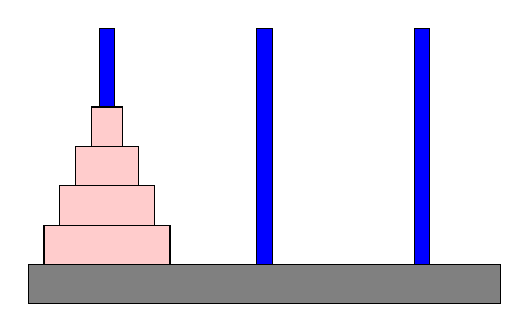
\begin{tikzpicture}
	%\draw[help lines] (0,0) grid (6,6);
	\draw[fill=blue, opacity=20] (0.9,0) rectangle (1.1,3);%poles
	\draw[fill=blue, opacity=20] (2.9,0) rectangle (3.1,3);%poles
	\draw[fill=blue, opacity=20] (4.9,0) rectangle (5.1,3);%poles


	\draw[fill=red!20!white, xshift=1cm, yshift=0cm] let 
		\p1=(-.8,0), \p2 = ($ -1*(\p1) + (0,0.5) $) 
	in 
	 (0,0) -- +(\p1) rectangle +(\p2);%first bar
	
	\draw[fill=red!20!white, xshift=1cm, yshift=0.5cm] let 
		\p1=(-.6,0), \p2 = ($ -1*(\p1) + (0,0.5) $) 
	in 
		(0,0) -- +(\p1) rectangle +(\p2);%first bar

	\draw[fill=red!20!white, xshift=1cm, yshift=1cm] let 
	\p1=(-.4,0), \p2 = ($ -1*(\p1) + (0,0.5) $) 
	in 
	(0,0) -- +(\p1) rectangle +(\p2);%first bar	 

	\draw[fill=red!20!white, xshift=1cm, yshift=1.5cm] let 
	\p1=(-.2,0), \p2 = ($ -1*(\p1) + (0,0.5) $) 
	in 
	(0,0) -- +(\p1) rectangle +(\p2);%first bar	 

	 
	\draw[fill=gray] (0,0) rectangle (6,-0.5);
\end{tikzpicture}
\end{center}


Here is the goal:

\begin{center}
	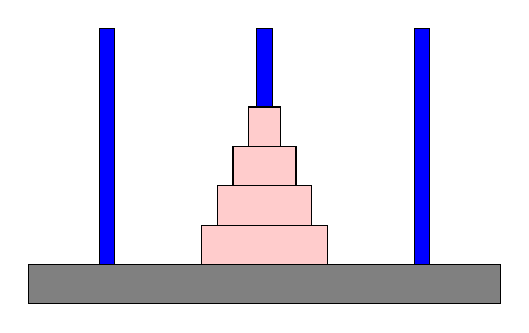
\begin{tikzpicture}
%\draw[help lines] (0,0) grid (6,6);
\draw[fill=blue, opacity=20] (0.9,0) rectangle (1.1,3);%poles
\draw[fill=blue, opacity=20] (2.9,0) rectangle (3.1,3);%poles
\draw[fill=blue, opacity=20] (4.9,0) rectangle (5.1,3);%poles


\draw[fill=red!20!white, xshift=3cm, yshift=0cm] let 
\p1=(-.8,0), \p2 = ($ -1*(\p1) + (0,0.5) $) 
in 
(0,0) -- +(\p1) rectangle +(\p2);%first bar

\draw[fill=red!20!white, xshift=3cm, yshift=0.5cm] let 
\p1=(-.6,0), \p2 = ($ -1*(\p1) + (0,0.5) $) 
in 
(0,0) -- +(\p1) rectangle +(\p2);%first bar

\draw[fill=red!20!white, xshift=3cm, yshift=1cm] let 
\p1=(-.4,0), \p2 = ($ -1*(\p1) + (0,0.5) $) 
in 
(0,0) -- +(\p1) rectangle +(\p2);%first bar	 

\draw[fill=red!20!white, xshift=3cm, yshift=1.5cm] let 
\p1=(-.2,0), \p2 = ($ -1*(\p1) + (0,0.5) $) 
in 
(0,0) -- +(\p1) rectangle +(\p2);%first bar	 


\draw[fill=gray] (0,0) rectangle (6,-0.5);
\end{tikzpicture}
\end{center}


The question is how many move do we need to move $n$ disk($T(n)$).


After you have played it for a couple games we will find that the strategy for moving $n$ disks is
\begin{enumerate}[1)]
	\item First, we need to move $n-1$ smallest disks to another pole first, this takes $T(n-1)$ turns.
	
	\begin{center}
			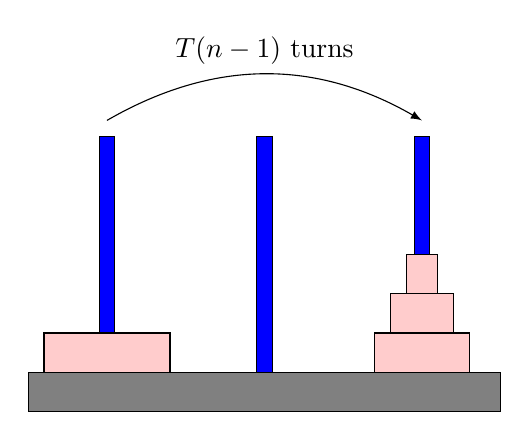
\begin{tikzpicture}[>=latex]
		%\draw[help lines] (0,0) grid (6,6);
		\draw[] (1,3.2) edge[bend left,->] node[above]() {$T(n-1)$ turns} (5,3.2) ;
		\draw[fill=blue, opacity=20] (0.9,0) rectangle (1.1,3);%poles
		\draw[fill=blue, opacity=20] (2.9,0) rectangle (3.1,3);%poles
		\draw[fill=blue, opacity=20] (4.9,0) rectangle (5.1,3);%poles
		
		
		\draw[fill=red!20!white, xshift=1cm, yshift=0cm] let 
		\p1=(-.8,0), \p2 = ($ -1*(\p1) + (0,0.5) $) 
		in 
		(0,0) -- +(\p1) rectangle +(\p2);%first bar
		
		\draw[fill=red!20!white, xshift=5cm, yshift=0cm] let 
		\p1=(-.6,0), \p2 = ($ -1*(\p1) + (0,0.5) $) 
		in 
		(0,0) -- +(\p1) rectangle +(\p2);%first bar
		
		\draw[fill=red!20!white, xshift=5cm, yshift=0.5cm] let 
		\p1=(-.4,0), \p2 = ($ -1*(\p1) + (0,0.5) $) 
		in 
		(0,0) -- +(\p1) rectangle +(\p2);%first bar	 
		
		\draw[fill=red!20!white, xshift=5cm, yshift=1.0cm] let 
		\p1=(-.2,0), \p2 = ($ -1*(\p1) + (0,0.5) $) 
		in 
		(0,0) -- +(\p1) rectangle +(\p2);%first bar	 
		
		
		\draw[fill=gray] (0,0) rectangle (6,-0.5);
		\end{tikzpicture}
	\end{center}
	
	\item Then we move the largest disk to the the desired pole. This takes 1 turn.
	
	\begin{center}
		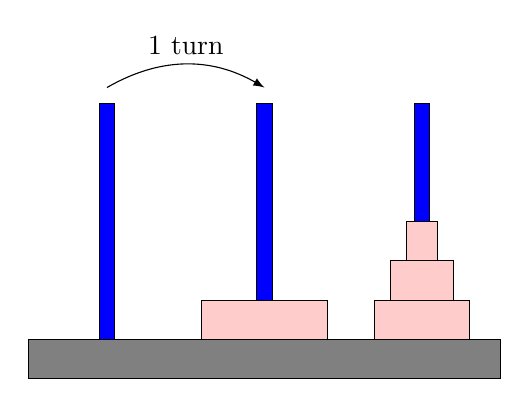
\begin{tikzpicture}[>=latex]
		%\draw[help lines] (0,0) grid (6,6);
		\draw[] (1,3.2) edge[bend left,->] node[above]() {$1$ turn} (3,3.2) ;
		\draw[fill=blue, opacity=20] (0.9,0) rectangle (1.1,3);%poles
		\draw[fill=blue, opacity=20] (2.9,0) rectangle (3.1,3);%poles
		\draw[fill=blue, opacity=20] (4.9,0) rectangle (5.1,3);%poles
		
		
		\draw[fill=red!20!white, xshift=3cm, yshift=0cm] let 
		\p1=(-.8,0), \p2 = ($ -1*(\p1) + (0,0.5) $) 
		in 
		(0,0) -- +(\p1) rectangle +(\p2);%first bar
		
		\draw[fill=red!20!white, xshift=5cm, yshift=0cm] let 
		\p1=(-.6,0), \p2 = ($ -1*(\p1) + (0,0.5) $) 
		in 
		(0,0) -- +(\p1) rectangle +(\p2);%first bar
		
		\draw[fill=red!20!white, xshift=5cm, yshift=0.5cm] let 
		\p1=(-.4,0), \p2 = ($ -1*(\p1) + (0,0.5) $) 
		in 
		(0,0) -- +(\p1) rectangle +(\p2);%first bar	 
		
		\draw[fill=red!20!white, xshift=5cm, yshift=1.0cm] let 
		\p1=(-.2,0), \p2 = ($ -1*(\p1) + (0,0.5) $) 
		in 
		(0,0) -- +(\p1) rectangle +(\p2);%first bar	 
		
		
		\draw[fill=gray] (0,0) rectangle (6,-0.5);
		\end{tikzpicture}
	\end{center}
		
	\item Lastly, we move the $n-1$ smallest disk to the desire pole.
	
	\begin{center}
		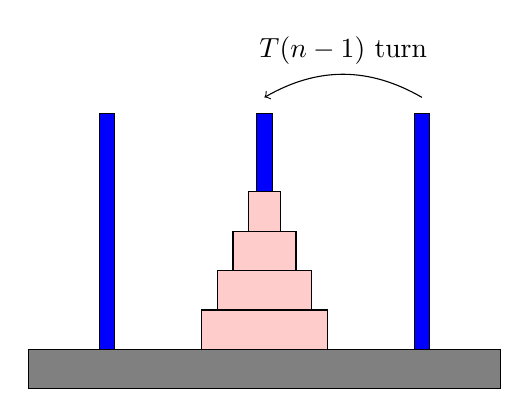
\begin{tikzpicture}
		%\draw[help lines] (0,0) grid (6,6);
		\draw[] (3,3.2) edge[bend left,<-] node[above]() {$T(n-1)$ turn} (5,3.2) ;
		\draw[fill=blue, opacity=20] (0.9,0) rectangle (1.1,3);%poles
		\draw[fill=blue, opacity=20] (2.9,0) rectangle (3.1,3);%poles
		\draw[fill=blue, opacity=20] (4.9,0) rectangle (5.1,3);%poles
		
		
		\draw[fill=red!20!white, xshift=3cm, yshift=0cm] let 
		\p1=(-.8,0), \p2 = ($ -1*(\p1) + (0,0.5) $) 
		in 
		(0,0) -- +(\p1) rectangle +(\p2);%first bar
		
		\draw[fill=red!20!white, xshift=3cm, yshift=0.5cm] let 
		\p1=(-.6,0), \p2 = ($ -1*(\p1) + (0,0.5) $) 
		in 
		(0,0) -- +(\p1) rectangle +(\p2);%first bar
		
		\draw[fill=red!20!white, xshift=3cm, yshift=1cm] let 
		\p1=(-.4,0), \p2 = ($ -1*(\p1) + (0,0.5) $) 
		in 
		(0,0) -- +(\p1) rectangle +(\p2);%first bar	 
		
		\draw[fill=red!20!white, xshift=3cm, yshift=1.5cm] let 
		\p1=(-.2,0), \p2 = ($ -1*(\p1) + (0,0.5) $) 
		in 
		(0,0) -- +(\p1) rectangle +(\p2);%first bar	 
		
		
		\draw[fill=gray] (0,0) rectangle (6,-0.5);
		\end{tikzpicture}
	\end{center}
\end{enumerate}

So, the total number of turn needed to move $n$ turn is
\[
	T(n) = 2T(n-1) +1
\]

The relation above does not really love like we have solve the problem. But, actually we did. If we can figure out how many move to move 1 disk($T(1)$) then we can get the number of turn to move 2 disks($T(2)$). With $T(2)$ we can get $T(3)$ and so on.

Finding $T(1)$ is quite easy we need exactly one step to solve the hanoi tower problem of $n$ disk. So the complete description of $T(n)$ is
\[
T(n) = 2T(n-1) +1; T(1)=1
\]

This formula is not very convenient for calculating how many turns we need. We want a closed form formula.

\section*{Plug and chug}

This is the brute force way that I really want you to be able to do. The strategy is just write it out and see the pattern. The problem is
\[
	T(n) = 2T(n-1) + 1; T(1) = 1
\]

Let us try to figure out the value of $T_5$. For this method is is very important that you \emph{do not simplify}. The pattern is usually lost if you simply each step.
\begin{align*}
	T_5 &= 2T_{4} +1 \\
	&= 2(2T_{3} + 1) +1\\
	&= 2^2T_{3} + 2 + 1\\
	&= 2^2(2T_{2} + 1) + 2 + 1\\
	&= 2^3T_{2} + 2^2 + 2 + 1\\
	&= 2^3(2T_{1}+1) + 2^2 + 2 + 1\\
	&= 2^4T_{1} + 2^3 + 2^2 + 2 + 1\\
	&= 2^4 + 2^3 + 2^2 + 2 + 1
\end{align*}

After serveral number of step you can guess that
\[
	T_n = 2^{n-1} + 2^{n-2} + \ldots + 2^2 + 2^1 + 1
\]

This sum is just the geometric sum we have learned before:
\[
	T_n = \frac{2^{n-1+1}-1}{2-1} = 2^n -1 
\]

This method is in no way proving that this is the solution. We just guess. To prove it you need to do induction. Watch carefully though the proof is a bit subtle. We have two definitions of hopefully the same function. We want to show that $T^*_n = 2^n + 1$ we found from plug and chuck and $T_n$ defined by the recurrence is the same function. So all we need to show is that $T_n$ and $T_n^*$ are equal for every single $n$.

\theorem $T_n^* = 2^n -1$ is equal to $T_n$ defined by $$T_n = 2T_{n-1} + 1; \forall n \ge 1$$ with $T_1=1$

\proof We will prove this by induction.
\predicate

	P(s):= $T_s^* == T_s$

\basecase $T_1^* = 2^1 -1 = 1$ and $T_1=1$ so $T_1 = T_1^*$ \checkmark

\inductivestep Here we assume that $T_k^* = T_k$ for some k.

Now we want to show that $T_{k+1}^* = T_{k+1}$

The left hand side can be found from the definiton of $T_n^*$
\[
	LHS = T_{k+1}^* = 2^{k+1} -1
\]

The right hand side we use the definition of $T_n = 2T(n-1) +1$. Then we use the IH that $T_{k} \expl{=}{IH} T_k^* \expl{=}{*def} 2^k - 1 $
\begin{align*}
	RHS &= T_{k+1}\\
	&= 2T_k + 1 & \text{Definition of $T_n$}\\
	&= 2T^*_k +1 & \text{By IH}\\
	&= 2\left(2^k - 1\right)+1 & \text{By Definition of $T^*_n$}\\
	&=2^{k+1} -2 +1\\
	&= 2^{k+1} - 1
\end{align*}

So, for all these reason we know that with all these assumptions
\[
	RHS = T_{k+1} = 2^{k+1} -1
\]
which is the same thing as the left hand side. Thus,
\[
	T_{k+1}^* = T_{k+1}
\]

So, by mathematical induction, $T_n = T_n^*$ for all $n \ge 1$. This means $T_n$ and $T_n^*$ is the same function.
\qedd

\section*{Some simple ones}
As a practice try to write a recurrence for the following situations
\begin{enumerate}
	\item Today I have no money. On everyday, I'll have one Baht more than what I had the day before. 
	\item I have 100 Baht today. At the end of every year I'll have the amount I had in the previous year plus the interest rate of $2\%$ on the amount I had last year. Plus, I'll put in another 100 Baht.
\end{enumerate}

\section*{Linear Recurrence}
Consider the following problem of counting the number of ways to walk up the $n$ step stairs. We have two choices
\begin{enumerate}
	\item We could walk 1 step up.
	\item Or, we could hop 2 steps up.
\end{enumerate}

For example, for 4 step stairs. We could
\begin{enumerate}[1.]
	\item step step step step.
	\item hop hop.
	\item step step hop
	\item hop step step
	\item step hop step
\end{enumerate}
There are 5 in total.

We can break the problem of counting down to smaller problems. The number of ways to walk up $n$ step stairs can be computer by
\begin{align*}
	\text{\# of ways for n step} = &\text{\# of way if we step first}\\ 
	&+ \text{\# of way if we hop first}
\end{align*}

If we step first, then we need to solve for the number of ways to step up n-1 step. If we hop first, then we need to solve for the number of ways to step up n-2 step. At least we have smaller problem to solve. So, we can write this a a recurrence
\[
	T_n = T_{n-1} + T_{n-2}
\]

We will also need a first few number to lock down all the subsequent numbers. We can just compute the number of wasy to step up 0 step and 1 step both are 1. So the complete description of the recurrence is

\[
	T_n = T_{n-1} + T_{n-2}; T_0 =1, T_1=1
\]

Of course this is the fibbonacci you have seen before many times in the homework.

This time we want to find the closed form formula for $T_n$. You can try plug and chug but, trust me, it won't get anywhere. I would be proud of you though if that is the first thing you try at least you are not afraid of brute forcing. We need a smarter way to solve this: GUESS for the solution.

Let us try to plug in $T^*(n) = x^n$ and hope that we can find $x$ that make $T^*$ at least satisfy the recurrence.

If $T^*(n) = x^n$ satisfy the recurrence that means
\begin{align*}
	x^n &= x^{n-1} + x^{n-2}\\
	x^2 &= x + 1\\
	x^2 -x -1 &= 0\\
\end{align*}
This equation is called the \kwd{characteristic equation}.
\begin{align*}
	x &= \frac{1 \pm \sqrt{1^2 +4}}{2}\\
	&= \frac{1 + \sqrt{5}}{2}, \frac{1 - \sqrt{5}}{2} 
\end{align*}

From this we know that
\[
	f(n) = \left(\frac{1 + \sqrt{5}}{2}\right)^n = a^n
\]
and 
\[
	g(n) = \left(\frac{1 - \sqrt{5}}{2}\right)^n = b^n
\]
solves the recurrence we want.

However, there is a bad news. Neither $f$ nor $g$ is the function we want. If we plugin, $n=1$ we should get 1. But, none of the solution we had give us the value we want for $n=1$.

\section*{Linear Homogeneous Recurrence}

But, we are not done yet. The recurrence we are solving is an example of a class of  recurrence called linear homogeneneous recurrence.

\definition A \kwd{linear homogeneous} recurrence is a recurrence of the form
\[
	f(n) + a_1 f(n-1) + a_2f(n-2) + \ldots +a_d f(n-d) = 0
\]

For example, the recurrence we are trying solve can be written in this form as
\[
	T(n) - T(n-1) - T(n-2) = 0.
\]
Not all recurrence is linear homogeneous recurrence. For instance, the recurrence we solve for the hanoi tower.
\[
	T(n) = 2T(n-1) + 1
\]
is not a linear homogeneous recurrence since if we move the $2T(n-1)$ terms to the left hand side. We are left with 1 not 0.

Linear Homogeneous recurrence has a very nice property that if we have 2 solution then the linear combination of the two solution is another solution. If you have a chance to study ODE you will see the same trick again.
\end{multicols} 
\theorem Let $f_n$ and $g_n$ be solution to a linear homogeneous recurrence:
\[
T(n) + a_1 T(n-1) \ldots +a_d T(n-d) = 0.
\]
Then, for all $r,s \in \real$, $r f_n + s g_n$ also solve the recurrence.

\proof The proof is quite straight forward. All we need to do is to plug the linear combination into the recurrence and see if it is equal to 0.

Plugging $r f(n) + s g(n)$ in to the recurrence gives
\begin{align*}
	LHS &= [r f_n + s g_n ] + a_1 [r f_{n-1} + s g_{n-1} ] + \ldots a_d [r f_{n-d} + s g_{n-d} ]\\
	& = r[f_n + a_1 f_{n-1} + \ldots a_df_{n-d}] + s[g_n + a_1 g_{n-1} + \ldots a_dg_{n-d}] & \text{collecting terms}\\
	& = r 0 + s 0 & \text{since $f_n,g_n$ solve the recurrence.}\\
	&=0
\end{align*}

So, this means $r f_n + s g_n$ solves the recurrence
\qedd
\begin{multicols}{2}

\section*{Initial Conditions}

The theorem we just prove is very useful for fitting the boundary conditions. So far for the stair problem we have 2 solutions but none of the fit the initial conditions. Any linear combination of the two is guaranteed to solve the recurrence. If we can find the linear combination that can satisfy the initial conditions then we are done.

The initial condition we need to satisfy are $T(0)=1$, $T(1)=1$. So, we hope that for some $a, b \in Real$
\begin{align*}
	r f_0 + s g_0 &= 1\\
	r f_1 + s g_1 &= 1
\end{align*}

The relation above implies
\begin{align}
	r + s &= 1\\
	r \frac{1 + \sqrt{5}}{2} + s \frac{1 - \sqrt{5}}{2}  &= 1.
\end{align}
This is just two equation with two unknown we can solve for $r$ and $s$. This yields
\begin{align*}
r &= \frac{1}{\sqrt{5}}\times \frac{1 + \sqrt{5}}{2}\\
s &= -\frac{1}{\sqrt{5}}\times \frac{1 - \sqrt{5}}{2}
\end{align*}

This means that the function that solve the recurrence and the initial condition is
\[
	h_n = \frac{1}{\sqrt{5}}\times \left(\frac{1 + \sqrt{5}}{2}\right)^{n+1} - \frac{1}{\sqrt{5}}\times \left(\frac{1 - \sqrt{5}}{2}\right)^{n+1},
\]
similar to what you prove in the homework(the initial condition is a bit different). This formula is called the Binet's formula.

Of course, this is no way a proof that is indeed a solution. We still need to show that this is true using induction. You have done that already in the homework.

\section*{Putting it together}
Since there were so many digression along the way of getting the solution. Let us do it again in one swoop to get the whole picture.

Let us try to solve the follwing recurrence
\[
	T(n) = -2 T(n-1) + 15 T(n-2)
\]
with the initial conditions
\[
T(0) = 1, T(1)=2
\]

First we guess that $T(n) = x^n$
\[
	x^n = -2x^{n-1} + 15 x^{n-2}
\]
This means the characteristic equation is
\[
	x^2 + 2x -15 = 0
\]
This can be factorized in to
\[
	(x-3)(x+5) = 0
\]
Thus, $f(n)=3^n$ and $g(n)=(-5)^n$ solves the recurrence.

Now we need to fit the initial conditions so we need to find $r,s \in \real$ such that
\begin{align*}
	r f(0) + s g(0) &= 1\\
	r f(1) + s g(1) &= 2\\
\end{align*}

The equations that we need to solve is
\begin{align*}
	r + s &= 1\\
	3r -5s &= 2
\end{align*}

Solving this yields$\displaystyle r = \frac{7}{8}$ and $\displaystyle s = \frac{1}{8}$. So, the solution to the recurrence is
\[
	T(n) = \frac{7}{8}3^n +\frac{1}{8}(-5)^n
\]

\section*{Double Root and What not}
Read the book if you are interested in what we should do if we got a double root.

%\section*{Merge Sort}
%Suppose you work part time as a librarian assistant. Each day you have big stack of returned books you need to put back to the corresponding shelf. To make putting back the book a bit less painful, you decide to sort it first.
%
%It is a standard for in the industry to charge by the number of comparison they need to make. For simplicity, let the standard price for 1 comparison be 1 Baht.
%
%Now you decide how much you should charge
%
%
%But, you are super lazy and try to use money to solve problem. So you decide to hire two subcontractor and assign each one of them to sort half of the books(randomly picked). You plan to merge the result of two later.
%
%
%The two subcontractor does not want to sort it either. So they each one of them hire two more subsub contractor to sort half of the workload they got. They only plan to merge



\section*{Maximum Buy/Sell Profit}
After you graduate, you become CEO of an big investment firm. You have many many employee. You have list of stock price for $n$ days(really big $n~10^5$) and you want to find the best time to buy stock then the best day to sell it later. Each of your employee is required by law to compare no more than 1 pair of number a day. Otherwise, you firm have to face labor abuse lawsuit. You want to get this done in 1 day. You want to decide how many people you need.

So, you call your three managers and ask them what to do.

Your first manager said all you need to do is to compute the profit for ever pair of buy and sell date. You will need to compute $n(n-1)$ profit and compare all of them to find the maximum. This requires $n(n-1)$ comparisons. So you will need around $10^{10}$ people. You fired this manager right away since there are only 7billion people on the earth.

Your second manager said all you need to do is to give the first half to one of the manager then give the second half to another manager. Ask them for the best date of each half. Three things can happen
\begin{enumerate}
	\item The best pair is in the first half.
	\item The best pair is in the second half.
	\item The best buy date is in the first half and the best sell date is in the second half. To compute this one we will just need to find the miminum of the first half and the maximum of the second half. This takes $(n-1)$ comparisons.
\end{enumerate}
Then, we need to compare the three this take 2 comparisons.

Of course, we do not know how many comparison the first two steps need. We know they are not going to do $n^2$ like the first manager since they will get fired right away. They will have to copy the way the second manger suggest by giving half of their work load to another group of people and hire another group to combine the result like we did. Then all the other manager will just copy your strategy recursively.\footnote{You can actually do much better than this by having the function returns max and min but we will not get there.
	}

This doesn't really help us count. The number of comparison need to solve the problem of size $n$ is
\[
	T(n) = \expl{T(n/2)}{First half} + \uexpl{T(n/2)}{second half} + \underbrace{n-1+2}_{\text{combine}}
\]

Like the previous recurrence the description is not complete description if we do not have the initial condition. If the list is has only 2 points then, we will just return that point as the maximum profit(potentially loss). So we have $T(2) = 1$

So, we have a recurrence relation.
\[
T(n) = 2T(n/2) + n + 1; T(2) = 1
\]

This means you can find $T(2)$, $T(4)$, $T(8)$ \ldots and so on. Let us try to solve this

\section*{Plug and Chug 2}
Since we go by down by 2 all the times so let
\[
	n = 2^k
\]
This means
\[
k = \log_2 n
\]
You should \kwd{always} try $2^k$. This will simplify the pattern a lot. 

Let us compute $T(2^5)$. Again we do not want to simplify since it will break the pattern.
\begin{align*}
	T(2^5) &= 2 T(2^4) + 2^5 + 1\\
	& = 2(2T(2^3) + 2^4 + 1) + 2^5 + 1\\
	& = 2^2 T(2^3) +  2^5 + 2 + 2^5 + 1\\
	& = 2^2(2T(2^2) + 2^3 + 1) + 2^5 + 2 + 2^5 + 1\\
	& = 2^3T(2^2) + 2^5 + 2^2 + 2^5 + 2 + 2^5 + 1\\
	& = 2^3(2T(2^1) + 2^2 + 1) + 2^5 + 2^2 + 2^5 + 2 + 2^5 + 1\\
	& = 2^4T(2^1) + 2^5 + 2^3 + 2^5 + 2^2 + 2^5 + 2 + 2^5 + 1\\
	& = \red{2^4} + \blue{2^5} + \red{2^3} + \blue{2^5} + \red{2^2} + \blue{2^5} + \red{2} + \blue{2^5} + \red{1}\\
	& = \red{2^4}  + \red{2^3}  + \red{2^2} + \red{2} + \red{1} + \blue{2^5} + \blue{2^5} + \blue{2^5} + \blue{2^5}\\
	& = \red{\sum_{i=0}^{i=5-1}2^i} + \blue{(5-1) 2^5}
\end{align*}
So, we can guess make that
\begin{align*}
	T(n) = T(2^k) &= \sum_{i=0}^{i=k-1} 2^i + (k-1) 2^k\\
	& = \frac{2^k - 1}{2-1} + (k-1)2^k & \text{Geo sum.}\\
	& = 2^k - 1 + k2^k - 2^k\\
	& = k2^k -1\\
	& = nk -1 & n = 2^k\\
	& = n \log_2 n - 1 & k = \log_2 n
\end{align*}

Of course this is not a proof. It is just a really good way of finding what to prove. You will need to do induction to verify this.


\section*{Rounding}

You may ask what happen to the number that is not $2^n$ for example $T(3)$. You can read the book. The rounding doesn't do much to the divide and conquer recurrence. You can usually just ignore it if all you need is just the asymptotic behavior. Trust me on this.
\end{multicols}

\section*{Drawing Tree}
Another way to solve divide and conquer recurrence is to draw workload tree. Where you have the actual work done by each manager/node written on it. Then all we have to do is to sum it up systematically. You will need to be a bit careful on where to end whether it is $k$ or $k-1$. To figure that out you usually need to plug in a specific number.
\begin{center}
\begin{tikzpicture}[level/.style={sibling distance=60mm/#1+5mm}]
\node [circle,draw] (z){$n+1$}
child {node [circle,draw] (a) {$\frac{n}{2}+1$}
	child {node [circle,draw] (b) {$\frac{n}{2^2}+1$}
		child {node {$\vdots$}
			child {node [circle,draw] (d) {$T_2=1$}}
			child {node [circle,draw] (e) {$1$}}
		} 
		child {node {$\vdots$}}
	}
	child {node [circle,draw] (g) {$\frac{n}{2^2}+1$}
		child {node {$\vdots$}}
		child {node {$\vdots$}}
	}
}
child {node [circle,draw] (j) {$\frac{n}{2}+1$}
	child {node [circle,draw] (k) {$\frac{n}{2^2}+1$}
		child {node {$\vdots$}}
		child {node {$\vdots$}}
	}
	child {node [circle,draw] (l) {$\frac{n}{2^2}+1$}
		child {node {$\vdots$}}
		child {node (c){$\vdots$}
			child {node [circle,draw] (o) {$1$}}
			child {node [circle,draw] (p) {$1$}
				child [grow=right] {node (q) {$=$} edge from parent[draw=none]
					child [grow=right] {node (q) {$n$} edge from parent[draw=none]
						child [grow=up] {node (r) {$\vdots$} edge from parent[draw=none]
							child [grow=up] {node (s) {$4\times(\frac{n}{4}+1)$} edge from parent[draw=none]
								child [grow=up] {node (t) {$2\times(\frac{n}{2}+1)$} edge from parent[draw=none]
									child [grow=up] {node (u) {$n+1$} edge from parent[draw=none]}
								}
							}
						}
						%child [grow=down] {node (v) {$O(n \cdot \lg n)$}edge from %parent[draw=none]}
					}
				}
			}
		}
	}
};
\path (a) -- (j) node [midway] {+};
\path (b) -- (g) node [midway] {+};
\path (k) -- (l) node [midway] {+};
\path (k) -- (g) node [midway] {+};
\path (d) -- (e) node [midway] {+};
\path (o) -- (p) node [midway] {+};
%\path (o) -- (e) node (x) [midway] {$\cdots$}
%child [grow=down] {
%	node (y) {$O\left(\displaystyle\sum_{i = 0}^k 2^i \cdot \frac{n}{2^i}\right)$}
%	edge from parent[draw=none]
%};
\path (q) -- (r) node [midway] {+};
\path (s) -- (r) node [midway] {+};
\path (s) -- (t) node [midway] {+};
\path (s) -- (l) node [midway] {=};
\path (t) -- (u) node [midway] {+};
\path (z) -- (u) node [midway] {=};
%\path (j) -- (t) node [midway] {=};
%\path (y) -- (x) node [midway] {$\Downarrow$};
%\path (v) -- (y)
%node (w) [midway] {$O\left(\displaystyle\sum_{i = 0}^k n\right) = O(k \cdot n)$};
%\path (q) -- (v) node [midway] {=};
%\path (e) -- (x) node [midway] {+};
%\path (o) -- (x) node [midway] {+};
%\path (y) -- (w) node [midway] {$=$};
%\path (v) -- (w) node [midway] {$\Leftrightarrow$};
%\path (r) -- (c) node [midway] {$\cdots$};
\end{tikzpicture}
\end{center}
All we need to find is the num of all the number in the node
\begin{align*}
	Sum &= \expl{\sum_{i=0}^{i=k-2}\left({n + 2^i}\right)}{all the terms before the last level} + \uexpl{\frac{n}{2}}{last level}\\ 
	&=(k-1)n + \sum_{i=0}^{i=k-2}2^i + \frac{n}{2}\\
	&= kn -n + 2^{k-1} - 1 + \frac{n}{2}\\
	&= kn - \cancel{n} + \cancel{\frac{n}{2}} -1 +\cancel{\frac{n}{2}}\\
	& = kn -1\\
	& = n\log_2 n -1
\end{align*}


Which is the same thing as what we found before. This method requires you to be a bit careful in getting the bound of the sum correct. Pick whichever method you like.

\section*{Josephus's Problem}

You can read about Josephus from wikipedia he is quite a character and a writer. What we are considering here will be a variant of Josephus problem. Consider $n$ prisoner standing in a circle starting from position 1 to position $n$.

\begin{center}
	\begin{tikzpicture}
	\draw[gray, dashed] (0,0) circle (2cm);
	\node()[] at (0:2cm) {1};
	\node()[] at (27:2cm) {2};
	\node()[] at (55:2cm) {3};
	\node()[] at (83:2cm) {4};
	\node()[] at (110:2cm) {5};
	\node()[] at (138:2cm) {6};
	\node()[] at (166:2cm) {7};
	\node()[] at (193:2cm) {8};
	\node()[] at (221:2cm) {9};
	\node()[] at (249:2cm) {10};
	\node()[] at (276:2cm) {11};
	\node()[] at (304:2cm) {12};
	\node()[] at (332:2cm) {13};	
	\end{tikzpicture}
\end{center}

The executor start skip the one prisoner then kill one then skip one and keep repeating the process until only one survivor is left.

For example, given the 13 prisoners. The first round of execution will kill out all the even-numbered people.

\begin{align*}
	1,\xcancel{2},3,\xcancel{4},5,\xcancel{6},7,\xcancel{8},9,\xcancel{10},11,\xcancel{12},13
\end{align*}

Then the next after skipping 13 the excutor then proceed to kill $1$ skip $3$ and kill $5$

\begin{align*}
\xcancel{1},3,\xcancel{5},7,\xcancel{9},11,\xcancel{13}
\end{align*}

After killing 13 the executor proceed to skip $3$ and kill $7$

\begin{align*}
3, \xcancel{7}, 11
\end{align*}

Then he skips $11$ and kill $3$

\begin{align*}
	\xcancel{3}, 11
\end{align*}

which means 11 survives.

The question is where do you want to stand if there are $n$ people? Let us consider this problem as a recurrence problem. First, we are going to consider the case where there are even number of people $n = 2k$. After the first round of executor. We will be left with $k = n/2$ people standing in a circle. Position 1 will have person number $1$. Position 2 will have person number $3$ on it and so on.

\begin{verbatim}
1, 2, 3, 4, 5 ,6 ,7, 8, 9, 10
1, 3, 5, 7, 9 
\end{verbatim}

If we happen to be able to figure out which position is safe for smaller circle we can infer about the safe position of the larger circle. Let the safe position for circle of $n$ people be $T_n$. If $n$ is even, we can ask our friend to find out which position is safe for circle of $n/2$ people, then all we need is translate that position to bigger circle.

\begin{align*}
	T_n = 2T_{n/2} - 1 \;\; \text{if $n$ is even.}
\end{align*}

The case where $n=2k+1$ is odd is similar to the even case except that the first person will be killed so we get rid of the first person and realign them. This means that ask our friend about the survival position for $(n-1)/2$ circle then translate the position for smaller circle to position for circle with $n$ people.

\begin{verbatim}
1, 2, 3, 4, 5 ,6 ,7, 8, 9, 10, 11
3, 5, 7, 9, 11
\end{verbatim}

This means

\begin{align*}
T_n = 2T_{(n-1)/2} + 1 \;\; \text{if $n$ is odd.}
\end{align*}

Combining the two gives us a funny recurrence.
\begin{align*}
	T_n = \begin{cases*}
	2T_{(n-1)/2} + 1 & \text{if $n$ is odd.}\\
	2T_{n/2} - 1 & \text{if $n$ is even.}
	\end{cases*}
\end{align*}

Writing down a few first values for $T_n$
\begin{verbatim}
1, 3, 1, 3, 5, 1, 3, 5, 7, 1, 3, 5, 7, 9, ...
\end{verbatim}
allows us to guess the solution. If $n = 2^m + l$ where $0 \le l < 2^m$ then $T_n = 2l + 1$. This can be proven quite easily by induction.










\end{document}
